\documentclass[tikz,border=0]{standalone}
\usepackage{xcolor}
\usepackage{tikz}

\begin{document}
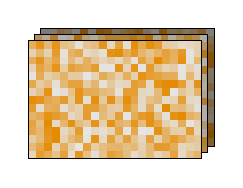
\begin{tikzpicture}[x=0.1cm,y=0.1cm]

\foreach \i in {0,...,21} {
  \foreach \j in {0,...,14} {

    \pgfmathsetmacro{\h}{rnd}

    \definecolor{cellcolor}{hsb}{0.1,\h,0.5}

    \fill[cellcolor] (\i,\j) rectangle ++(1,1);
  }
}

\draw[] (0, 0) rectangle (22, 15);

\foreach \i in {-0.8,...,20.2} {
  \foreach \j in {-0.8,...,13.2} {

    \pgfmathsetmacro{\h}{rnd}

    \definecolor{cellcolor}{hsb}{0.1,\h,0.7}

    \fill[cellcolor] (\i,\j) rectangle ++(1,1);
  }
}

\draw[] (-0.8, -0.8) rectangle (21.2, 14.2);

\foreach \i in {-1.6,...,19.4} {
  \foreach \j in {-1.6,...,12.4} {

    \pgfmathsetmacro{\h}{rnd}

    \definecolor{cellcolor}{hsb}{0.1,\h,0.9}

    \fill[cellcolor] (\i,\j) rectangle ++(1,1);
  }
}

\draw[] (-1.6, -1.6) rectangle (20.4, 13.4);

\end{tikzpicture}
\end{document}
